\documentclass{article}

\usepackage[utf8]{inputenc}
\usepackage{geometry}
\usepackage{listings}
\usepackage{graphicx}
\usepackage{geometry}
\usepackage{courier}

\graphicspath{{../images/}}

\title{HW 6 \\ Parallel Mandelbrot}
\author{Philip Nelson}
\date{2018 October 5}

\lstset{basicstyle=\footnotesize\ttfamily\normalsize,
        breaklines=true,
        stepnumber=1,
       }

\begin{document}

\maketitle

\section*{Introduction}

The purpose of this assignment is to write an MPI program that generates an image of the mandelbrot set as described by the set of complex numbers $c$ for which the function ${f_{c}(z)=z^{2}+c}$ does not diverge when iterated from $z=0$. My program takes as input the image height, image width, maximum number of iterations, minimum x/real value, maximum x/real value, and minimum y/imaginary value. Then in parallel, it calculates the number of iterations every pixel in the image takes to diverge. The program uses the master-slave architecture to send tasks. The master sends rows to the slaves in a round-robbin style. The slaves calculate the iteration values for the pixels in each row they are assigned and send them back to the master. The master then receives each message and incorporates the message buffers into one array. When every pixel has been calculated, the array is converted to a PNG image, using libpng, based on a color scheme. Functionality to output to a ppm file is included.

\section*{Code}
The code is broken up into five main files, main.cpp, controller.cpp,  calculator.cpp, color.cpp, and writePNG.hpp. The files are included below.

\bigskip

\subsection{main.cpp}
\lstinputlisting[showstringspaces=false, language=c++, numbers=left]{../main.cpp}

\subsection{controller.cpp}
\lstinputlisting[showstringspaces=false, language=c++, numbers=left]{../controller.cpp}

\subsection{calculator.cpp}
\lstinputlisting[showstringspaces=false, language=c++, numbers=left]{../calculator.cpp}

\subsection{color.cpp}
\lstinputlisting[showstringspaces=false, language=c++, numbers=left]{../color.cpp}

\subsection{ppmToBmp.hpp}
\lstinputlisting[showstringspaces=false, language=c++, numbers=left]{../writePNG.hpp}
\newpage
\section*{Output}

\begin{lstlisting}[showstringspaces=false]

# mpic++ -std=c++17 -g0 -O3 -Wall -Wextra -Werror main.cpp calculator.cpp color.cpp -o mandelbrot.out

# mpiexec -n 4 ./mandelbrot.out 2048 2048 1000 -.760574 -.762574 -.0837596

Successfully wrote brot2048.png
2048 x 2048
Time to compute: 1.5373
Time to write image: 0.690633


3 finished, completed 683 lines of the image
2 finished, completed 684 lines of the image
1 finished, completed 684 lines of the image

\end{lstlisting}

\section*{Findings}

I generated the image below, Figure \ref{fig:image}, as a 256x256, 512x512, 1024x2014, 2048x2048, 4096x4096, and 8192x8192 pixel image. I ran each size 10 times and took the average time to calculate the number of iterations for each pixel and the time to write the file to the disk. The results are detailed in Figure \ref{fig:graph}. The graph shows that the time to generate an image increases with the square of the number of pixels. The same is true for the writing of the file to the disk. Another interesting metric can be seen in Figure: \ref{fig:graph2} which shows how the pixels per second calculated was not largely affected by the image size. You can however see that it slowly increases with larger images. I believe this is due to caching. The last metric observed is the speedup of the parallel version compared to the serial version. This relationship can be seen in Figure \ref{fig:graph3}. It can be observed that the speedup levels off with the size of the image. I think that the speedup is lower at first because the image is so small that sending messages is more overhead than it is worth. Then you get more speedup with larger images because there are so many more pixels. 

\begin{figure}[!htbp]
    \centering
    \fbox{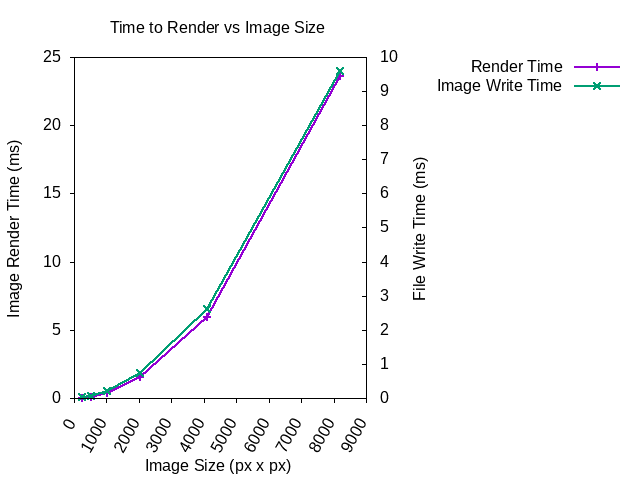
\includegraphics[width=150mm]{benchmark.png}}%tabe size
    \caption{}
    \label{fig:graph}
\end{figure}

\begin{figure}[!htbp]
    \centering
    \fbox{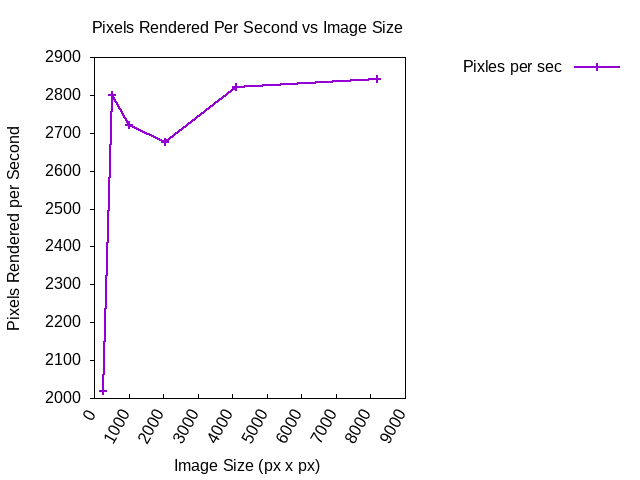
\includegraphics[width=150mm]{pixelsPerSec.png}}%tabe size
    \caption{}
    \label{fig:graph2}
\end{figure}

\begin{figure}[!htbp]
    \centering
    \fbox{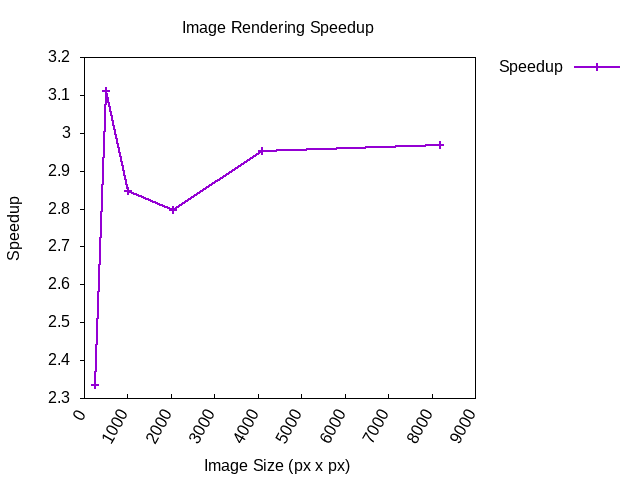
\includegraphics[width=150mm]{speedup.png}}%tabe size
    \caption{}
    \label{fig:graph3}
\end{figure}

\begin{figure}[!htbp]
    \centering
    \fbox{\includegraphics[width=150mm]{spiral8192.png}}%tabe size
    \caption{}
    \label{fig:image}
\end{figure}

\begin{figure}[!htbp]
    \centering
    \fbox{
\includegraphics[width=150mm]{spiral2048.png}}%tabe size
    \caption{}
    \label{fig:image}
\end{figure}

\begin{figure}[!htbp]
    \centering
    \fbox{
\includegraphics[width=150mm]{final.png}}%tabe size
    \caption{}
    \label{fig:image}
\end{figure}

\end{document}
